\documentclass{article}
\usepackage{iclr2027_conference,times}
%%%%% NEW MATH DEFINITIONS %%%%%

\usepackage{amsmath,amsfonts,bm}

% Mark sections of captions for referring to divisions of figures
\newcommand{\figleft}{{\em (Left)}}
\newcommand{\figcenter}{{\em (Center)}}
\newcommand{\figright}{{\em (Right)}}
\newcommand{\figtop}{{\em (Top)}}
\newcommand{\figbottom}{{\em (Bottom)}}
\newcommand{\captiona}{{\em (a)}}
\newcommand{\captionb}{{\em (b)}}
\newcommand{\captionc}{{\em (c)}}
\newcommand{\captiond}{{\em (d)}}

% Highlight a newly defined term
\newcommand{\newterm}[1]{{\bf #1}}


% Figure reference, lower-case.
\def\figref#1{figure~\ref{#1}}
% Figure reference, capital. For start of sentence
\def\Figref#1{Figure~\ref{#1}}
\def\twofigref#1#2{figures \ref{#1} and \ref{#2}}
\def\quadfigref#1#2#3#4{figures \ref{#1}, \ref{#2}, \ref{#3} and \ref{#4}}
% Section reference, lower-case.
\def\secref#1{section~\ref{#1}}
% Section reference, capital.
\def\Secref#1{Section~\ref{#1}}
% Reference to two sections.
\def\twosecrefs#1#2{sections \ref{#1} and \ref{#2}}
% Reference to three sections.
\def\secrefs#1#2#3{sections \ref{#1}, \ref{#2} and \ref{#3}}
% Reference to an equation, lower-case.
\def\eqref#1{equation~\ref{#1}}
% Reference to an equation, upper case
\def\Eqref#1{Equation~\ref{#1}}
% A raw reference to an equation---avoid using if possible
\def\plaineqref#1{\ref{#1}}
% Reference to a chapter, lower-case.
\def\chapref#1{chapter~\ref{#1}}
% Reference to an equation, upper case.
\def\Chapref#1{Chapter~\ref{#1}}
% Reference to a range of chapters
\def\rangechapref#1#2{chapters\ref{#1}--\ref{#2}}
% Reference to an algorithm, lower-case.
\def\algref#1{algorithm~\ref{#1}}
% Reference to an algorithm, upper case.
\def\Algref#1{Algorithm~\ref{#1}}
\def\twoalgref#1#2{algorithms \ref{#1} and \ref{#2}}
\def\Twoalgref#1#2{Algorithms \ref{#1} and \ref{#2}}
% Reference to a part, lower case
\def\partref#1{part~\ref{#1}}
% Reference to a part, upper case
\def\Partref#1{Part~\ref{#1}}
\def\twopartref#1#2{parts \ref{#1} and \ref{#2}}

\def\ceil#1{\lceil #1 \rceil}
\def\floor#1{\lfloor #1 \rfloor}
\def\1{\bm{1}}
\newcommand{\train}{\mathcal{D}}
\newcommand{\valid}{\mathcal{D_{\mathrm{valid}}}}
\newcommand{\test}{\mathcal{D_{\mathrm{test}}}}

\def\eps{{\epsilon}}


% Random variables
\def\reta{{\textnormal{$\eta$}}}
\def\ra{{\textnormal{a}}}
\def\rb{{\textnormal{b}}}
\def\rc{{\textnormal{c}}}
\def\rd{{\textnormal{d}}}
\def\re{{\textnormal{e}}}
\def\rf{{\textnormal{f}}}
\def\rg{{\textnormal{g}}}
\def\rh{{\textnormal{h}}}
\def\ri{{\textnormal{i}}}
\def\rj{{\textnormal{j}}}
\def\rk{{\textnormal{k}}}
\def\rl{{\textnormal{l}}}
% rm is already a command, just don't name any random variables m
\def\rn{{\textnormal{n}}}
\def\ro{{\textnormal{o}}}
\def\rp{{\textnormal{p}}}
\def\rq{{\textnormal{q}}}
\def\rr{{\textnormal{r}}}
\def\rs{{\textnormal{s}}}
\def\rt{{\textnormal{t}}}
\def\ru{{\textnormal{u}}}
\def\rv{{\textnormal{v}}}
\def\rw{{\textnormal{w}}}
\def\rx{{\textnormal{x}}}
\def\ry{{\textnormal{y}}}
\def\rz{{\textnormal{z}}}

% Random vectors
\def\rvepsilon{{\mathbf{\epsilon}}}
\def\rvtheta{{\mathbf{\theta}}}
\def\rva{{\mathbf{a}}}
\def\rvb{{\mathbf{b}}}
\def\rvc{{\mathbf{c}}}
\def\rvd{{\mathbf{d}}}
\def\rve{{\mathbf{e}}}
\def\rvf{{\mathbf{f}}}
\def\rvg{{\mathbf{g}}}
\def\rvh{{\mathbf{h}}}
\def\rvu{{\mathbf{i}}}
\def\rvj{{\mathbf{j}}}
\def\rvk{{\mathbf{k}}}
\def\rvl{{\mathbf{l}}}
\def\rvm{{\mathbf{m}}}
\def\rvn{{\mathbf{n}}}
\def\rvo{{\mathbf{o}}}
\def\rvp{{\mathbf{p}}}
\def\rvq{{\mathbf{q}}}
\def\rvr{{\mathbf{r}}}
\def\rvs{{\mathbf{s}}}
\def\rvt{{\mathbf{t}}}
\def\rvu{{\mathbf{u}}}
\def\rvv{{\mathbf{v}}}
\def\rvw{{\mathbf{w}}}
\def\rvx{{\mathbf{x}}}
\def\rvy{{\mathbf{y}}}
\def\rvz{{\mathbf{z}}}

% Elements of random vectors
\def\erva{{\textnormal{a}}}
\def\ervb{{\textnormal{b}}}
\def\ervc{{\textnormal{c}}}
\def\ervd{{\textnormal{d}}}
\def\erve{{\textnormal{e}}}
\def\ervf{{\textnormal{f}}}
\def\ervg{{\textnormal{g}}}
\def\ervh{{\textnormal{h}}}
\def\ervi{{\textnormal{i}}}
\def\ervj{{\textnormal{j}}}
\def\ervk{{\textnormal{k}}}
\def\ervl{{\textnormal{l}}}
\def\ervm{{\textnormal{m}}}
\def\ervn{{\textnormal{n}}}
\def\ervo{{\textnormal{o}}}
\def\ervp{{\textnormal{p}}}
\def\ervq{{\textnormal{q}}}
\def\ervr{{\textnormal{r}}}
\def\ervs{{\textnormal{s}}}
\def\ervt{{\textnormal{t}}}
\def\ervu{{\textnormal{u}}}
\def\ervv{{\textnormal{v}}}
\def\ervw{{\textnormal{w}}}
\def\ervx{{\textnormal{x}}}
\def\ervy{{\textnormal{y}}}
\def\ervz{{\textnormal{z}}}

% Random matrices
\def\rmA{{\mathbf{A}}}
\def\rmB{{\mathbf{B}}}
\def\rmC{{\mathbf{C}}}
\def\rmD{{\mathbf{D}}}
\def\rmE{{\mathbf{E}}}
\def\rmF{{\mathbf{F}}}
\def\rmG{{\mathbf{G}}}
\def\rmH{{\mathbf{H}}}
\def\rmI{{\mathbf{I}}}
\def\rmJ{{\mathbf{J}}}
\def\rmK{{\mathbf{K}}}
\def\rmL{{\mathbf{L}}}
\def\rmM{{\mathbf{M}}}
\def\rmN{{\mathbf{N}}}
\def\rmO{{\mathbf{O}}}
\def\rmP{{\mathbf{P}}}
\def\rmQ{{\mathbf{Q}}}
\def\rmR{{\mathbf{R}}}
\def\rmS{{\mathbf{S}}}
\def\rmT{{\mathbf{T}}}
\def\rmU{{\mathbf{U}}}
\def\rmV{{\mathbf{V}}}
\def\rmW{{\mathbf{W}}}
\def\rmX{{\mathbf{X}}}
\def\rmY{{\mathbf{Y}}}
\def\rmZ{{\mathbf{Z}}}

% Elements of random matrices
\def\ermA{{\textnormal{A}}}
\def\ermB{{\textnormal{B}}}
\def\ermC{{\textnormal{C}}}
\def\ermD{{\textnormal{D}}}
\def\ermE{{\textnormal{E}}}
\def\ermF{{\textnormal{F}}}
\def\ermG{{\textnormal{G}}}
\def\ermH{{\textnormal{H}}}
\def\ermI{{\textnormal{I}}}
\def\ermJ{{\textnormal{J}}}
\def\ermK{{\textnormal{K}}}
\def\ermL{{\textnormal{L}}}
\def\ermM{{\textnormal{M}}}
\def\ermN{{\textnormal{N}}}
\def\ermO{{\textnormal{O}}}
\def\ermP{{\textnormal{P}}}
\def\ermQ{{\textnormal{Q}}}
\def\ermR{{\textnormal{R}}}
\def\ermS{{\textnormal{S}}}
\def\ermT{{\textnormal{T}}}
\def\ermU{{\textnormal{U}}}
\def\ermV{{\textnormal{V}}}
\def\ermW{{\textnormal{W}}}
\def\ermX{{\textnormal{X}}}
\def\ermY{{\textnormal{Y}}}
\def\ermZ{{\textnormal{Z}}}

% Vectors
\def\vzero{{\bm{0}}}
\def\vone{{\bm{1}}}
\def\vmu{{\bm{\mu}}}
\def\vtheta{{\bm{\theta}}}
\def\va{{\bm{a}}}
\def\vb{{\bm{b}}}
\def\vc{{\bm{c}}}
\def\vd{{\bm{d}}}
\def\ve{{\bm{e}}}
\def\vf{{\bm{f}}}
\def\vg{{\bm{g}}}
\def\vh{{\bm{h}}}
\def\vi{{\bm{i}}}
\def\vj{{\bm{j}}}
\def\vk{{\bm{k}}}
\def\vl{{\bm{l}}}
\def\vm{{\bm{m}}}
\def\vn{{\bm{n}}}
\def\vo{{\bm{o}}}
\def\vp{{\bm{p}}}
\def\vq{{\bm{q}}}
\def\vr{{\bm{r}}}
\def\vs{{\bm{s}}}
\def\vt{{\bm{t}}}
\def\vu{{\bm{u}}}
\def\vv{{\bm{v}}}
\def\vw{{\bm{w}}}
\def\vx{{\bm{x}}}
\def\vy{{\bm{y}}}
\def\vz{{\bm{z}}}

% Elements of vectors
\def\evalpha{{\alpha}}
\def\evbeta{{\beta}}
\def\evepsilon{{\epsilon}}
\def\evlambda{{\lambda}}
\def\evomega{{\omega}}
\def\evmu{{\mu}}
\def\evpsi{{\psi}}
\def\evsigma{{\sigma}}
\def\evtheta{{\theta}}
\def\eva{{a}}
\def\evb{{b}}
\def\evc{{c}}
\def\evd{{d}}
\def\eve{{e}}
\def\evf{{f}}
\def\evg{{g}}
\def\evh{{h}}
\def\evi{{i}}
\def\evj{{j}}
\def\evk{{k}}
\def\evl{{l}}
\def\evm{{m}}
\def\evn{{n}}
\def\evo{{o}}
\def\evp{{p}}
\def\evq{{q}}
\def\evr{{r}}
\def\evs{{s}}
\def\evt{{t}}
\def\evu{{u}}
\def\evv{{v}}
\def\evw{{w}}
\def\evx{{x}}
\def\evy{{y}}
\def\evz{{z}}

% Matrix
\def\mA{{\bm{A}}}
\def\mB{{\bm{B}}}
\def\mC{{\bm{C}}}
\def\mD{{\bm{D}}}
\def\mE{{\bm{E}}}
\def\mF{{\bm{F}}}
\def\mG{{\bm{G}}}
\def\mH{{\bm{H}}}
\def\mI{{\bm{I}}}
\def\mJ{{\bm{J}}}
\def\mK{{\bm{K}}}
\def\mL{{\bm{L}}}
\def\mM{{\bm{M}}}
\def\mN{{\bm{N}}}
\def\mO{{\bm{O}}}
\def\mP{{\bm{P}}}
\def\mQ{{\bm{Q}}}
\def\mR{{\bm{R}}}
\def\mS{{\bm{S}}}
\def\mT{{\bm{T}}}
\def\mU{{\bm{U}}}
\def\mV{{\bm{V}}}
\def\mW{{\bm{W}}}
\def\mX{{\bm{X}}}
\def\mY{{\bm{Y}}}
\def\mZ{{\bm{Z}}}
\def\mBeta{{\bm{\beta}}}
\def\mPhi{{\bm{\Phi}}}
\def\mLambda{{\bm{\Lambda}}}
\def\mSigma{{\bm{\Sigma}}}

% Tensor
\DeclareMathAlphabet{\mathsfit}{\encodingdefault}{\sfdefault}{m}{sl}
\SetMathAlphabet{\mathsfit}{bold}{\encodingdefault}{\sfdefault}{bx}{n}
\newcommand{\tens}[1]{\bm{\mathsfit{#1}}}
\def\tA{{\tens{A}}}
\def\tB{{\tens{B}}}
\def\tC{{\tens{C}}}
\def\tD{{\tens{D}}}
\def\tE{{\tens{E}}}
\def\tF{{\tens{F}}}
\def\tG{{\tens{G}}}
\def\tH{{\tens{H}}}
\def\tI{{\tens{I}}}
\def\tJ{{\tens{J}}}
\def\tK{{\tens{K}}}
\def\tL{{\tens{L}}}
\def\tM{{\tens{M}}}
\def\tN{{\tens{N}}}
\def\tO{{\tens{O}}}
\def\tP{{\tens{P}}}
\def\tQ{{\tens{Q}}}
\def\tR{{\tens{R}}}
\def\tS{{\tens{S}}}
\def\tT{{\tens{T}}}
\def\tU{{\tens{U}}}
\def\tV{{\tens{V}}}
\def\tW{{\tens{W}}}
\def\tX{{\tens{X}}}
\def\tY{{\tens{Y}}}
\def\tZ{{\tens{Z}}}


% Graph
\def\gA{{\mathcal{A}}}
\def\gB{{\mathcal{B}}}
\def\gC{{\mathcal{C}}}
\def\gD{{\mathcal{D}}}
\def\gE{{\mathcal{E}}}
\def\gF{{\mathcal{F}}}
\def\gG{{\mathcal{G}}}
\def\gH{{\mathcal{H}}}
\def\gI{{\mathcal{I}}}
\def\gJ{{\mathcal{J}}}
\def\gK{{\mathcal{K}}}
\def\gL{{\mathcal{L}}}
\def\gM{{\mathcal{M}}}
\def\gN{{\mathcal{N}}}
\def\gO{{\mathcal{O}}}
\def\gP{{\mathcal{P}}}
\def\gQ{{\mathcal{Q}}}
\def\gR{{\mathcal{R}}}
\def\gS{{\mathcal{S}}}
\def\gT{{\mathcal{T}}}
\def\gU{{\mathcal{U}}}
\def\gV{{\mathcal{V}}}
\def\gW{{\mathcal{W}}}
\def\gX{{\mathcal{X}}}
\def\gY{{\mathcal{Y}}}
\def\gZ{{\mathcal{Z}}}

% Sets
\def\sA{{\mathbb{A}}}
\def\sB{{\mathbb{B}}}
\def\sC{{\mathbb{C}}}
\def\sD{{\mathbb{D}}}
% Don't use a set called E, because this would be the same as our symbol
% for expectation.
\def\sF{{\mathbb{F}}}
\def\sG{{\mathbb{G}}}
\def\sH{{\mathbb{H}}}
\def\sI{{\mathbb{I}}}
\def\sJ{{\mathbb{J}}}
\def\sK{{\mathbb{K}}}
\def\sL{{\mathbb{L}}}
\def\sM{{\mathbb{M}}}
\def\sN{{\mathbb{N}}}
\def\sO{{\mathbb{O}}}
\def\sP{{\mathbb{P}}}
\def\sQ{{\mathbb{Q}}}
\def\sR{{\mathbb{R}}}
\def\sS{{\mathbb{S}}}
\def\sT{{\mathbb{T}}}
\def\sU{{\mathbb{U}}}
\def\sV{{\mathbb{V}}}
\def\sW{{\mathbb{W}}}
\def\sX{{\mathbb{X}}}
\def\sY{{\mathbb{Y}}}
\def\sZ{{\mathbb{Z}}}

% Entries of a matrix
\def\emLambda{{\Lambda}}
\def\emA{{A}}
\def\emB{{B}}
\def\emC{{C}}
\def\emD{{D}}
\def\emE{{E}}
\def\emF{{F}}
\def\emG{{G}}
\def\emH{{H}}
\def\emI{{I}}
\def\emJ{{J}}
\def\emK{{K}}
\def\emL{{L}}
\def\emM{{M}}
\def\emN{{N}}
\def\emO{{O}}
\def\emP{{P}}
\def\emQ{{Q}}
\def\emR{{R}}
\def\emS{{S}}
\def\emT{{T}}
\def\emU{{U}}
\def\emV{{V}}
\def\emW{{W}}
\def\emX{{X}}
\def\emY{{Y}}
\def\emZ{{Z}}
\def\emSigma{{\Sigma}}

% entries of a tensor
% Same font as tensor, without \bm wrapper
\newcommand{\etens}[1]{\mathsfit{#1}}
\def\etLambda{{\etens{\Lambda}}}
\def\etA{{\etens{A}}}
\def\etB{{\etens{B}}}
\def\etC{{\etens{C}}}
\def\etD{{\etens{D}}}
\def\etE{{\etens{E}}}
\def\etF{{\etens{F}}}
\def\etG{{\etens{G}}}
\def\etH{{\etens{H}}}
\def\etI{{\etens{I}}}
\def\etJ{{\etens{J}}}
\def\etK{{\etens{K}}}
\def\etL{{\etens{L}}}
\def\etM{{\etens{M}}}
\def\etN{{\etens{N}}}
\def\etO{{\etens{O}}}
\def\etP{{\etens{P}}}
\def\etQ{{\etens{Q}}}
\def\etR{{\etens{R}}}
\def\etS{{\etens{S}}}
\def\etT{{\etens{T}}}
\def\etU{{\etens{U}}}
\def\etV{{\etens{V}}}
\def\etW{{\etens{W}}}
\def\etX{{\etens{X}}}
\def\etY{{\etens{Y}}}
\def\etZ{{\etens{Z}}}

% The true underlying data generating distribution
\newcommand{\pdata}{p_{\rm{data}}}
% The empirical distribution defined by the training set
\newcommand{\ptrain}{\hat{p}_{\rm{data}}}
\newcommand{\Ptrain}{\hat{P}_{\rm{data}}}
% The model distribution
\newcommand{\pmodel}{p_{\rm{model}}}
\newcommand{\Pmodel}{P_{\rm{model}}}
\newcommand{\ptildemodel}{\tilde{p}_{\rm{model}}}
% Stochastic autoencoder distributions
\newcommand{\pencode}{p_{\rm{encoder}}}
\newcommand{\pdecode}{p_{\rm{decoder}}}
\newcommand{\precons}{p_{\rm{reconstruct}}}

\newcommand{\laplace}{\mathrm{Laplace}} % Laplace distribution

\newcommand{\E}{\mathbb{E}}
\newcommand{\Ls}{\mathcal{L}}
\newcommand{\R}{\mathbb{R}}
\newcommand{\emp}{\tilde{p}}
\newcommand{\lr}{\alpha}
\newcommand{\reg}{\lambda}
\newcommand{\rect}{\mathrm{rectifier}}
\newcommand{\softmax}{\mathrm{softmax}}
\newcommand{\sigmoid}{\sigma}
\newcommand{\softplus}{\zeta}
\newcommand{\KL}{D_{\mathrm{KL}}}
\newcommand{\Var}{\mathrm{Var}}
\newcommand{\standarderror}{\mathrm{SE}}
\newcommand{\Cov}{\mathrm{Cov}}
% Wolfram Mathworld says $L^2$ is for function spaces and $\ell^2$ is for vectors
% But then they seem to use $L^2$ for vectors throughout the site, and so does
% wikipedia.
\newcommand{\normlzero}{L^0}
\newcommand{\normlone}{L^1}
\newcommand{\normltwo}{L^2}
\newcommand{\normlp}{L^p}
\newcommand{\normmax}{L^\infty}

\newcommand{\parents}{Pa} % See usage in notation.tex. Chosen to match Daphne's book.

\DeclareMathOperator*{\argmax}{arg\,max}
\DeclareMathOperator*{\argmin}{arg\,min}

\DeclareMathOperator{\sign}{sign}
\DeclareMathOperator{\Tr}{Tr}
\let\ab\allowbreak

\usepackage[utf8]{inputenc}
\usepackage[T1]{fontenc}
\usepackage{graphicx}
\usepackage{booktabs}
\usepackage{amsmath,amssymb}
\usepackage{microtype}
\usepackage{url}
\usepackage{hyperref}
\hypersetup{hidelinks}

\title{Before Privatizing Evolution: Is There Enough Utility to Select?}
\author{Anonymous Authors}

% \iclrfinalcopy
\begin{document}
\maketitle

\begin{abstract}
 Test-time evolving LLM agents retain state and score candidate outputs, creating a plausible privacy channel and an apparent target for differential privacy (DP). Private selection matters, however, only if sensitive information persists, the score tracks semantic utility, and generation supplies useful alternatives. We audit these premises in a released multi-agent runtime on PlanCraft. A preregistered three-arm study detects no post-input canary exposure in 20 instances. Positive controls and measured state mutation make this a bounded failed-to-detect result, not evidence of non-leakage. The released score assigns 85\% weight to output length. Removing this term collapses score scale across DeepSeek and Qwen, but a synthesis of 42 paired runs gives an exactness change of only $+0.024$ with 95\% interval $[-0.095,0.143]$. More decisively, an oracle selector over recorded candidates has only 0--8.3 percentage points of headroom across four frozen cohorts. We then enlarge support prospectively on 20 untouched Qwen tasks. Five independent stochastic trajectories within the same runtime instead of one add 1.00 unique canonical plan $[0.50,1.60]$ and raise executable-oracle accuracy from 0.60 to 0.80, at three times the token cost. A stopped DeepSeek repair gate reveals task-level response collapse on two selected hard failures: one invalid response occupies 86.25\% and 95\% of 80 conditioned calls. A frozen same-task control reverses our initial explanation: under public-task-only prompts, these rates rise to 98.75\% and 95\%, with 0/160 executable. This task/model near-determinism is not attributable to repair conditioning. These results establish a practical order of operations for private evolving systems: demonstrate a persistent channel, validate the optimized signal, measure support headroom, and only then calibrate private selection.
\end{abstract}

\section{Introduction}

LLM agents increasingly adapt while solving a task. They revise role prompts, summarize memories, assign contribution scores, and change workflows or communication structure. TacoMAS exemplifies this design: a fast loop produces and evaluates agent outputs, while a slower controller can update feedback and topology \citep{xu2026tacomas}. Such systems invite a natural privacy proposal. If an input can enter persistent evolved state, privatize the scores or decisions that update that state.

This proposal joins two questions that need not have the same answer. A mechanism can provide a valid event-level DP guarantee for a bounded score while protecting a decision with negligible task value. Conversely, a useful candidate selector says nothing about whether natural-language memories and messages are private. Before measuring a privacy--utility frontier, three empirical premises must hold:
\begin{enumerate}
    \item sensitive information measurably enters post-input persistent state
    \item the score being privatized causally tracks executable utility
    \item the realized candidate pool contains a better output worth selecting.
\end{enumerate}
Architecture diagrams do not establish any of them. A model may fail to retain a tested secret over a short horizon. A ``contribution'' score may mostly reward verbose text. A perfect selector cannot recover a candidate the generator never produced.

We develop a persistence-aware executable audit around these premises and apply it to a frozen TacoMAS runtime on PlanCraft, a tool-using crafting benchmark with deterministic action-list evaluation \citep{dagan2025plancraft}. The audit changed the research question. We did not observe the motivating post-input canary channel in the preregistered setting, and removing the dominant score term did not reliably improve exactness. The bottleneck instead lay upstream: most failed runs contained no executable candidate for any selector to recover.

 That observation yields a phenomenon--remedy--escape arc. Fixed-pool selection is empirically bounded: across four frozen cohorts, an oracle over all persisted candidates improves accuracy by at most 0--8.3 points. The cheapest obvious remedy, repeatedly repairing a candidate under fixed execution feedback, can collapse onto the same wrong response despite stochastic decoding. Independent trajectories within this runtime expand task-relevant support and raise the pool oracle by 20 points, making selector-level DP worth analyzing, although at substantial cost.

Our contributions are:
\begin{itemize}
    \item a three-gate audit separating persistent exposure, signal validity, and candidate support
    \item a realized-pool upper bound that applies to every private or non-private selector restricted to the recorded candidates
     \item prospective evidence that independent generation expands support beyond the fixed-pool bound, with a matched-slot analysis locating the gain in cross-context coverage
    \item a diagnosis of \emph{task-level response collapse} on two selected hard failures: nominal decoding stochasticity need not create useful diversity with or without repair context.
\end{itemize}
We do not present a new end-to-end private agent. The result is a measurement framework and a constructive test of when private selection becomes worth studying.

\section{Auditing Evolving-Agent Selection}

\subsection{Persistent exposure after the input disappears}

At round $t$, agent $v$ has persistent text-bearing state
\[
s_{v,t}=(\phi_{v,t},m_{v,t},f_{v,t},o_{v,t},q_{v,t}),
\]
covering policy text, memory, feedback, stored outputs, and score history. A canary placed in the round-one query trivially occurs in that query and may be echoed immediately. We therefore define leakage operationally as exact or preregistered five-token partial recovery from persistent state at rounds 3 or 5, after the direct-input checkpoint.

The audit uses three five-round arms: evolution with a canary, a depth-matched reset that restores initial state after each round, and evolution without a canary. The reset control distinguishes persistence created by state evolution from ordinary processing of a repeated task. Structural graph edits are disabled so that all arms have the same three-agent topology and depth. We snapshot every declared text channel, store only match metadata in research artifacts, and separately verify the extractor by deterministic channel injection and a live memory-write positive control.

\subsection{Signal validity before privacy calibration}

The released non-slow-round score is
\[
c(y,e)=0.85\min\{1,|y|/800\}+0.15\mathbf 1\{e=\mathrm{success}\}.
\]
Length can therefore move the score much more than environment success. To distinguish correlation from consequence, we prospectively compare the released score with a length-zero arm while holding prompts, topology, rounds, feedback opportunities, and structural masks fixed. References are withheld until generation finishes, and deterministic executable exactness is computed offline. This firewall prevents an evaluator from leaking the answer into stopping, retention, or feedback.

For a randomized score intervention $Z$, define its arm-level utility consequence as
\[
\widehat\delta_U^{\mathrm{abl}}=
\widehat{\mathbb E}[U\mid Z=1]-\widehat{\mathbb E}[U\mid Z=0].
\]
This randomized-arm diagnostic asks whether the intervention changes downstream utility. It is not a parameter of a candidate selector. For two candidates with utility-score gap $g_U^{\mathrm{sel}}=u(c^+)-u(c^-)$ and candidate-score sensitivity $\Delta_u$, define the separate local selector ratio $\rho_U^{\mathrm{sel}}=g_U^{\mathrm{sel}}/\Delta_u$. Private discrimination depends on $\varepsilon\rho_U^{\mathrm{sel}}$. For a monotone exponential mechanism over $k$ candidates, the preferred-candidate probability is
\[
\frac{1}{1+(k-1)e^{-\varepsilon\rho_U^{\mathrm{sel}}}}.
\]
If the intervention changes scores but not utility, increasing $\varepsilon$ cannot make the targeted signal useful.

\subsection{Candidate-pool headroom}

Let $f_i$ be run $i$'s final answer and let $\mathcal C_i$ contain $f_i$ plus all persisted round-agent candidates available to a downstream selector. For executable utility $U$, define
\[
H_i=\max_{c\in\mathcal C_i}U(c)-U(f_i).
\]
$H_i$ is an exact upper bound for the realized run: no selector whose output must belong to $\mathcal C_i$ can improve by more than $H_i$. This includes noisy maximum, the exponential mechanism, and any non-private reranker over the same support. The bound does not constrain regeneration, repair, or new tool interaction because those operations change $\mathcal C_i$.

We parse candidate text into canonical crafting plans and execute it without reference answers. The reference sequence is retained only for offline secondary checks. This distinction matters because a plausible explanation is not a successful plan, while an executable candidate with different surface text is useful.

\subsection{Inference and experimental sequence}

Paired binary effects use task-level risk differences, paired task bootstraps, and exact discordant-pair tests when positive and negative differences are both possible. Nested pools satisfy $C_1\subset C_5$, so their support and oracle differences cannot be negative. We report task-bootstrap intervals and one-sided lower bounds, not sign-test $p$-values. Provider calls, rounds, candidate slots, and repeated repairs are never treated as independent task units.

The experiments proceed in a fixed order. We first audit canary exposure and cached score validity with DeepSeek V4 Flash. We then replicate the length ablation on a non-degenerate DeepSeek cohort and an untouched Qwen3.7-Max cohort. A zero-call oracle audit measures fixed-pool headroom. Finally, a prospective Qwen study expands candidate support with independent trajectories, followed by a compute-matched DeepSeek gate comparing an independent restart with direct executor-guided repair. Protocols, stopping rules, amendments, and provider-accounting details appear in the appendix.

\section{Results}

\subsection{The leakage and score premises do not pass their gates}

All 60 cells in the 20-instance canary study complete five rounds. We detect no exact or five-token partial canary in post-input persistent state in any arm (Table~\ref{tab:audit}). The evolve-arm one-sided 95\% upper confidence bound is 13.9\%, so the result cannot exclude a rare or modest exposure rate. The extractor recovers 7/7 deterministic channel injections and a live canary written into memory at round 2. State is active rather than inert: 617/720 comparable agent transitions change, all 168 recorded slow-feedback fields are nonempty, and retention fires in 60/300 rounds. The defensible result is therefore \emph{failed to detect with a functioning instrument}.

\begin{table}[t]
\caption{The first two gates. Exposure is measured only after the input round. Length ablations report length-zero minus released-score exactness.}
\label{tab:audit}
\centering
\small
\begin{tabular}{lccc}
\toprule
Study & $n$ & Primary observation & 95\% interval \\
\midrule
Canary: evolve & 20 & exact/partial $0/20$ & upper bound 0.139 \\
Canary: reset & 20 & exact/partial $0/20$ & upper bound 0.139 \\
DeepSeek initial ablation & 10 pairs & exactness $0.000$ & $[0,0]$ \\
DeepSeek healthy cohort & 12 pairs & exactness $+0.167$ & $[0,0.417]$ \\
Qwen healthy cohort & 20 pairs & exactness $-0.050$ & $[-0.250,0.150]$ \\
Stratified synthesis & 42 pairs & exactness $+0.024$ & $[-0.095,0.143]$ \\
\bottomrule
\end{tabular}
\end{table}

The score audit also corrects a tempting overstatement. Maximum score has AUC 0.755 for final exactness in the original 60 runs, but only five runs are exact and those successes come from three task instances. Scores at least 0.8 occur mostly in failed runs only because failures dominate the cohort. Relative to base rate, high scores are mildly enriched among successes.

Randomized intervention supplies the causal result. Removing length sharply reduces mean contribution score in every study: from 0.429 to 0.069 in the initial DeepSeek pairs, by $-0.308$ $[-0.381,-0.230]$ in the non-degenerate DeepSeek replication, and by $-0.117$ $[-0.150,-0.084]$ in Qwen. It also eliminates every score at least 0.8 in the paired cohorts. Exactness does not move consistently (Table~\ref{tab:audit}). The pooled direction is near zero, and the two healthy-regime point estimates have opposite signs. Length controls the released score scale, but deleting it is not a validated utility improvement.

\subsection{Fixed-pool selection has little realized headroom}

We execute the final answer and every persisted round-agent candidate in four independently frozen original or control cohorts. Table~\ref{tab:headroom} reports the final accuracy and candidate-pool oracle. In every cohort, average headroom is between zero and 8.3 points. This is not a confidence statement about all future tasks. It is an exact statement about what any selector could have recovered from each recorded pool.

\begin{table}[t]
\caption{Executable headroom for selectors restricted to persisted candidates. Intervals resample tasks within cohort. DeepSeek X1 has $n=13$ because forward execution cannot certify the seven \texttt{IMPOSSIBLE} references. Diversity summaries retain all 20 evolve runs.}
\label{tab:headroom}
\centering
\small
\begin{tabular}{lcccc}
\toprule
Cohort & $n$ & Final & Oracle & $\widehat H$ [95\% interval] \\
\midrule
DeepSeek X1 evolve & 13 & .154 & .154 & .000 $[0,0]$ \\
DeepSeek healthy evolve & 12 & .500 & .583 & .083 $[0,.250]$ \\
DeepSeek retention control & 20 & .000 & .050 & .050 $[0,.150]$ \\
Qwen released score & 20 & .550 & .600 & .050 $[0,.150]$ \\
\bottomrule
\end{tabular}
\end{table}

Pooling the four heterogeneous original/control cohorts gives 3 recoverable failures among 65 semantically eligible runs. The two-sided Clopper--Pearson interval is $[0.010,0.129]$ only under an exchangeable-Bernoulli reading. The cohort-stratified bootstrap interval is $[0,0.108]$. These population intervals do not alter the exact realized-pool bound.

The Qwen audit makes the failure mode concrete. Of nine failed final answers under released scoring, only one run contains an executable intermediate candidate. The other eight are generation failures. The length-zero arm similarly has one recoverable failure and nine generation failures. Most failed runs are not cases where a good candidate was scored badly. No good candidate exists on the recorded surface.

Literal duplication is model-dependent and therefore not the general explanation. Qwen repeats exact text in roughly 81--82\% of its 16 slots, whereas DeepSeek duplicate-text rates are much lower. Task-relevant support is small in both model families: across selected arms, 38/72 runs contain no parseable canonical plan, 22 contain one, eight contain two, and only four contain at least three. The common bottleneck is effective executable support, not identical wording.

\subsection{Independent contexts expand support}

We test the bound's escape clause prospectively on 20 untouched Qwen length-two tasks. Each task receives one temperature-zero trajectory and five independent temperature-0.7 trajectories. Every five-round trajectory supplies 15 agent outputs and a final answer. After canonical deduplication, $C_j$ is the nested union of the temperature-zero trajectory and the first $j$ stochastic trajectories.

Moving from $C_1$ to $C_5$ adds 1.00 canonical plan per task, with two-sided task-bootstrap interval $[0.50,1.60]$ and one-sided 95\% lower bound 0.60. Executable-oracle accuracy rises from 0.60 to 0.80, a gain of 0.20 $[0.05,0.40]$. Because these pools are nested, we do not report sign-test $p$-values. A non-nested comparison between the first temperature-0.7 trajectory and the temperature-zero trajectory finds a support difference of $-0.05$ $[-0.35,0.25]$. Temperature alone is not sufficient. The measured gain comes from accumulating independent trajectories.

At a matched 16 candidate slots, sampling across the five stochastic trajectories yields expected oracle coverage 0.626, compared with 0.570 for 16 slots within one trajectory. The difference is 0.056 $[0.016,0.105]$. This cached comparison locates useful diversity across independently restarted contexts, not merely across more token draws within one shared context. It does not isolate a multi-agent advantage because every trajectory uses the same three-agent runtime.

The final answers alone expose the same allocation effect: an oracle over five independent stochastic finals reaches 0.65, compared with 0.570 for 16 slots sampled within one trajectory. Within this runtime, independent restarts therefore contribute more observed coverage than adding rounds and agents inside a shared trajectory, but this comparison does not identify an architectural multi-agent effect.

The gain is uneven. Across the 100 stochastic trajectories, per-task success estimates are exactly zero or one for 14/20 tasks. Four tasks are rescued by $C_5$ but not $C_1$, and three of these contain a valid plan in only one of five trajectories. A fresh-draw plug-in expectation is 0.751 at five stochastic trajectories, whereas the realized nested $C_5$ pool reaches 0.80 on the same sample. The former averages estimated future draws, while the latter is the observed cached pool. The plug-in curve rises to 0.798 at twenty and has an empirical asymptote of 0.80, but this is finite-sample extrapolation. Zero successes in five trials still permits a one-sided 95\% binomial upper bound of 0.451, so 0.80 is not an identified hard ceiling.

The escape is also expensive. $C_1$ records 4.81M tokens and $C_5$ 14.43M, a 3.00-fold increase for a 0.20 oracle gain. Independent restarting is an existence proof and a cost baseline, not an efficient method.

\begin{figure}[t]
\centering
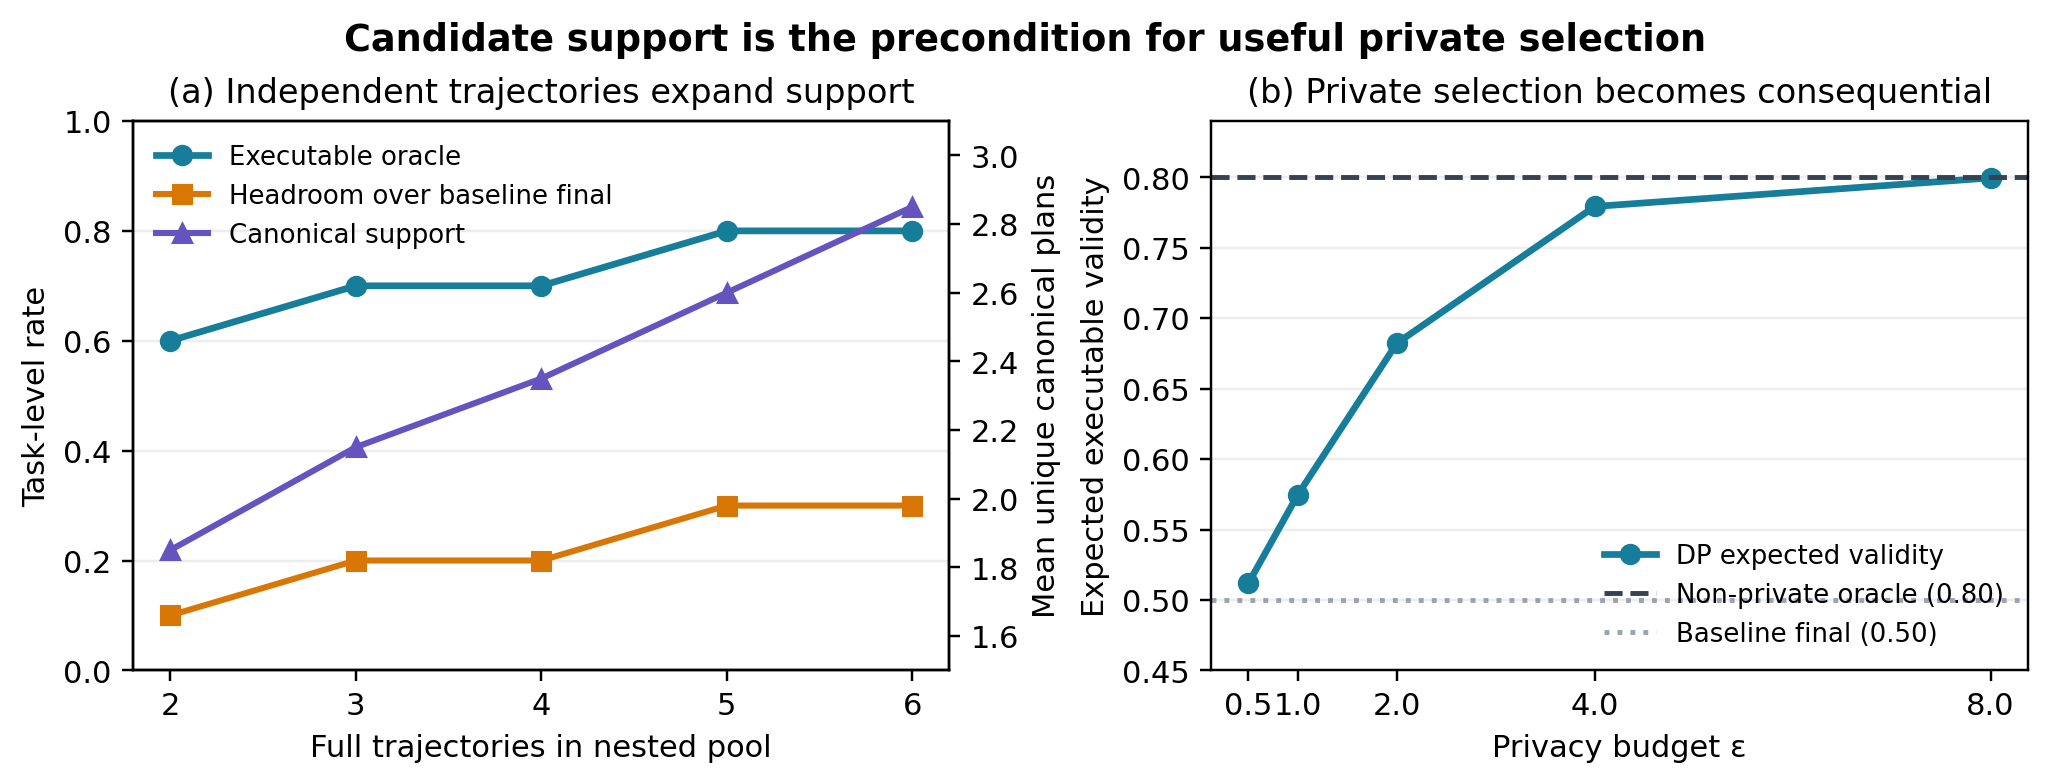
\includegraphics[width=0.95\linewidth]{figures/qwen-candidate-pool-enlargement.png}
\caption{Independent trajectories enlarge canonical support and executable headroom. The selector-level DP curve is meaningful only after the pool contains mixed-validity alternatives. The dashed 0.80 line is the cached-pool oracle, not end-to-end private-system accuracy.}
\label{fig:pool}
\end{figure}

\subsection{The obvious cheap remedy does not diversify hard failures}

We next ask whether direct repair can beat the restart baseline without paying for another full trajectory. Eight untouched DeepSeek tasks first receive one shared temperature-zero trajectory. If its pool succeeds, both methods stop. Otherwise, one arm runs a full temperature-0.7 restart, whose realized token use caps sequential temperature-0.7 repairs in the other arm. Repair receives the public task, its current candidate, and reference-free execution diagnostics.

Five of eight anchors already succeed, leaving only three informative failures rather than the preregistered minimum of four. The gate stops and no main cohort runs. Among those three failures, restart succeeds on 0/3 and repair on 1/3, with one discordant task and exact paired $p=1$. On the rescued task, repair succeeds on its first 1,008-token call while the matched-budget restart fails after 157,910 tokens, an existence result on one task rather than an efficiency ratio.

The two exhausted repairs tell a different story. On TEST0030, 69/80 calls return the identical invalid string \texttt{["IMPOSSIBLE"]}. After semantic normalization, 78/80 express impossibility. TEST0535 returns \texttt{["redstone\_torch"]} in 76/80 calls, repeatedly omitting the required intermediate. Thus nominally stochastic decoding under a fixed task, candidate, and diagnostic context concentrates on one wrong answer at raw modal rates of 86.25\% and 95\%.

We froze a same-task control before making another provider call. DeepSeek then received only the public task and the same output-format instruction, with no current candidate, executor diagnostic, attempt index, or response history. TEST0030 returned \texttt{["bookshelf"]} in 79/80 calls (98.75\%). TEST0535 returned raw \texttt{["redstone\_torch"]} in 76/80 calls and the same semantic plan in 80/80. None of the 160 public-task-only responses was executable. The mean task-level conditioned-minus-public-only raw modal-rate difference is $-0.0625$.

This control reverses our initial explanation. Conditioning is not necessary for the concentration and does not increase it on either selected task. We therefore use \emph{task-level response collapse}: direct stochastic generation remains trapped on one invalid endpoint under both prompts. The repeated calls estimate two within-task response distributions, not 160 task units, so the result does not estimate a population prevalence. It nevertheless explains why raising temperature inside a direct prompt can add almost no support while full independent trajectories sometimes escape.

\begin{figure}[t]
\centering
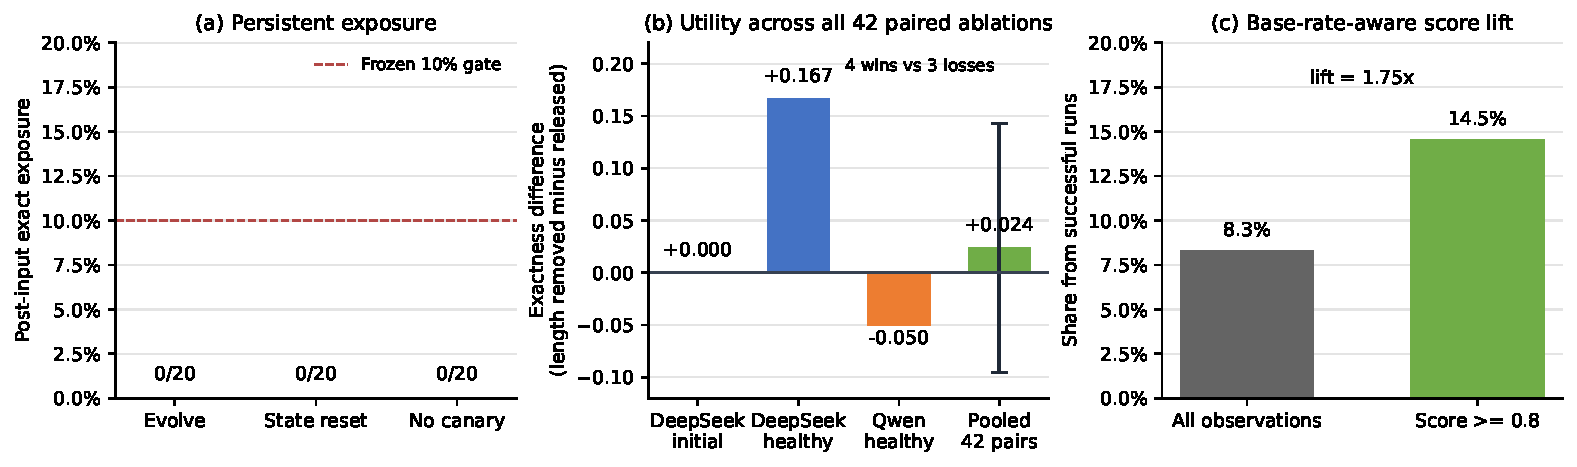
\includegraphics[width=0.96\linewidth]{figures/evolution-audit-main-results.pdf}
\caption{Secondary audit results. Post-input exposure is not detected. The 42-pair utility synthesis combines all three length interventions rather than only the initial cohort, and the original score has modest base-rate-aware lift.}
\label{fig:audit}
\end{figure}

\subsection{Private selection becomes non-vacuous only after support expands}

On a mixed $C_5$ pool, trusted binary executor utility has $g_U^{\mathrm{sel}}=\Delta_u=1$ and hence local $\rho_U^{\mathrm{sel}}=1$. Under candidate-score replacement adjacency, the monotone exponential mechanism samples index $j$ with probability proportional to $\exp(\varepsilon u_j/\Delta_u)$. Its mean executable probability is 0.512, 0.575, 0.682, 0.779, and 0.800 at $\varepsilon=0.5,1,2,4,8$, respectively, against the non-private oracle of 0.80. At $\varepsilon=0.5$, 0.512 is barely above the 0.50 baseline. The curve becomes materially separated near $\varepsilon=2$ in this binary-gap setting.

This is a selector-level theory check, not end-to-end privacy for the agent. Candidate texts, prompts, memories, inter-agent messages, and control flow remain trusted. Only the released selected index or output is covered by the stated adjacency. The curve nevertheless illustrates the audit's purpose. Before pool expansion, many failures offer no valid-versus-invalid choice and DP calibration governs a nearly vacuous decision. After expansion, the same mechanism protects a release with measurable utility at stake.

\section{Implications and Related Work}

Test-time optimization uses language models as optimizers or textual-gradient generators \citep{yang2023opro,yuksekgonul2024textgrad}. Self-consistency, tree search, and compute-aware inference instead spend additional test-time computation on diverse samples or structured exploration \citep{wang2022selfconsistency,yao2023tot,zhou2023lats,snell2024testtime}. Our headroom measurement complements this literature by asking a prior question: before optimizing search or selection, did the recorded generator expose any executable alternative?

Feedback-based agents such as ReAct, Reflexion, Self-Refine, and LATS condition later generation on actions, evaluation, or verbal memory \citep{yao2022react,shinn2023reflexion,madaan2023selfrefine,zhou2023lats}. Multi-agent sampling and layered aggregation seek gains from multiple response sources \citep{li2024moreagents,wang2024moa,xu2026tacomas}. Our matched-slot result distinguishes independent-context coverage from additional slots within one trajectory. The repair gate and public-only control show the same wrong mode under feedback-conditioned and direct prompts. Context independence is therefore an empirical variable, not an automatic consequence of temperature.

Learned evaluation can track preferences while exhibiting position, self-enhancement, and verbosity biases \citep{zheng2023judge}. Length-controlled evaluation directly targets the latter confound \citep{dubois2024length}. We instead intervene on a score used inside an evolving runtime and measure machine-executable utility. The separation between score movement and task movement is therefore causal and operational, not only a meta-evaluation correlation.

Canary methods test whether rare secrets influence model outputs \citep{carlini2019secret}. Our adaptation targets retained test-time state rather than trained parameters and separates immediate echo from later exposure. Work on indirect prompt injection, memory poisoning, tool-using-agent attacks, and privacy-norm behavior demonstrates that agent state and external observations can carry security- or privacy-relevant information \citep{greshake2023indirect,chen2024agentpoison,debenedetti2024agentdojo,shao2024privacylens}. These threat models motivate measurement but do not imply that our specific canary must persist.

Differential privacy calibrates randomized releases to sensitivity \citep{dwork2006calibrating,dwork2014foundations}. Report Noisy Max \citep{dwork2014foundations}, the exponential mechanism \citep{mcsherry2007mechanism}, and selection from candidates whose score functions are themselves private \citep{liu2019private} cover distinct private-selection settings. Private prompt optimization \citep{hong2024dpopt} and continual-observation tools \citep{dwork2010continual} protect other bounded channels, but formal privacy does not establish that the protected decision improves task outcomes.

The observed support bottleneck also changes the engineering target. Better reranking cannot solve generator-unreachable tasks. Independent restarts do, but at three times the token cost. Direct repair can exploit execution feedback and stop early, yet the stopped gate shows that stochastic generation can remain trapped on one invalid endpoint with or without repair conditioning. Refinement methods therefore cannot assume that feedback supplies diversity. Efficient diversity requires an intervention that changes task-relevant support without multiplying full trajectories. Designing and validating such an intervention is future work, not a post-hoc addition to this study.

An end-to-end private architecture would still need an explicit privacy principal, adjacency relation, public transcript, and trusted boundary. Natural-language memory, cross-agent messages, stopping time, and topology changes can reveal information independently of a private score. One possible direction is a typed-edge billboard design in which cross-boundary communication is mediated through a privatized summary and slow-loop actions are post-processing. The billboard lemma gives a standard route from a shared DP signal plus each participant's own data to joint DP outputs \citep{hsu2014private}. We do not evaluate that architecture here.

\section{Limitations}

The leakage audit covers one canary family, injection route, model, five-round horizon, and fixed topology. Topology evolution is disabled, so the study does not test leakage through structural edits. With 0/20 observations it cannot exclude rates below 13.9\% at one-sided 95\% confidence, and it does not mount adaptive extraction attacks. Qwen replicates the score intervention but not leakage.

PlanCraft exactness is deliberately strict and may ignore useful partial reasoning. The headroom result applies only to recorded candidates and binary target-reaching utility. Hidden reasoning, new repairs, and unrecorded tool interactions lie outside the bound. The four cohort estimates are modest in size, and their intervals do not justify a universal numerical ceiling.

An exploratory X2 diagnostic combines state verification with bounded action-distance filtering. It replays all seven feasible development tasks and, across two preselected held-out batches, 12/12 feasible tasks with 8/12 canonical exact plans; all six impossible-reference tasks trigger bounded stops. Symbolic search alone reproduces the held-out totals without model calls. Removing bounded pre-checks and distance filtering from the DeepSeek planner yields 8/12 feasible replays and 5/12 canonical plans on the same cohort. All four replay discordances favor symbolic search (two-sided exact $p=0.125$). These component controls locate executable coverage in the symbolic planning machinery without establishing an LLM or multi-agent advantage. The appendix reports them as post-hoc planning diagnostics, not confirmatory comparisons of the evolution arms.

The Qwen enlargement study has 20 tasks and one benchmark. Its nested design identifies added-pool gains but not a sign-symmetric treatment test. Its estimated trajectory curve assumes conditional i.i.d. restarts beyond the five observed. Cost totals are provider-recorded token counts rather than wall-clock or monetary comparisons. The matched-slot result identifies cross-trajectory coverage in the cached multi-agent runtime, not a causal multi-agent advantage.

Task-level response collapse is observed on two selected exhausted DeepSeek tasks. The public-task-only control removes candidate and diagnostic conditioning, but repeated calls still characterize only two tasks and do not create 160 independent task units. The stopped repair gate has three informative comparisons and one discordance, and the successful branch stops after one draw. Prevalence and association with success therefore remain unidentified.

Finally, the paper does not provide end-to-end DP. The selector experiment protects only a candidate-validity release under a narrow replacement adjacency. It leaves candidate text and the evolving transcript trusted.

\section{Conclusion}

Private selection in evolving LLM agents is consequential only when there is a persistent channel to protect, a utility-relevant signal to privatize, and useful generated support to select. In our audited setting, the first channel is not detected, removing the dominant score term does not reliably change utility, and fixed candidate pools leave at most 0--8.3 points of realized headroom. Independent trajectories raise the oracle from 0.60 to 0.80 but triple token use. Direct stochastic generation on two hard failures instead collapses onto one wrong endpoint even without repair context. These measurements turn a premature privacy mechanism question into a sharper systems question: how can evolving agents create independent, executable support efficiently enough that private selection is worth its budget?

\section*{Reproducibility Statement}

Every reported experiment has a frozen JSON protocol, resumable runner, machine-readable artifact, and closure manifest. References are withheld during online generation and exactness is recomputed offline. Repeated calls, trajectories, and candidate slots are clustered by task in uncertainty analyses. Raw canaries and provider credentials are excluded from research artifacts. The appendix records amendments, stopping decisions, excluded provider-error traces, and artifact locations.

\section*{AI Use Statement}

Generative AI tools assisted with research planning, code implementation, experiment orchestration, data analysis, and manuscript drafting. Reported numerical results were recomputed from stored artifacts and checked by automated tests. The authors take responsibility for the final content.

\bibliography{references}
\bibliographystyle{iclr2027_conference}

\appendix
\sloppy

This appendix preserves protocol and diagnostic details from the current main submission. All quantities are generated from the same frozen artifacts cited in the main paper.

\section{Reference-firewall calibration failure}

The initial reference-firewall implementation returned online quality zero for all expensive evaluations. The runtime stores a historical best candidate only when quality strictly improves over an initial value of zero. Constant-zero quality could therefore prevent candidate persistence independently of arm assignment. The issue was detected after the first pair and before interpreting its outcomes.

We froze an amendment that marked both cells \texttt{\detokenize{invalid_harness_calibration}}, excluded them from every endpoint and the 3M valid-token cap, retained them in the artifact, and replaced constant zero with the same reference-free text heuristic in both arms. The complete pair was then restarted. The invalid cells used 282,399 tokens; the 20 valid cells used 2,716,894 tokens and 1,083 calls; total observed use was 2,999,293 tokens. This near-miss demonstrates that reference isolation must cover control flow, not merely omit a reference-derived metric from the final table.

\section{Detailed null sensitivity}

The initial zero-exposure result in 20 evolve instances has an exact one-sided 95\% upper bound of 13.9\%. The completed replication has zero exposure in 120 evolve instances, lowering the corresponding bound to 2.5\%; the replication is the primary current estimate for this audited setting. A true event rate of 7.7\% already gives an 80\% chance of at least one observed event in the initial cohort. In the paired initial leakage comparison, six pure evolve-only discordances are required for two-sided exact \(p<0.05\), corresponding to a 30-point observed risk difference at \(n=20\). Under the explicit planning scenario of 5\% control risk and 10\% evolve risk with within-pair independence, power at 20 pairs is 1.7\% one-sided and 0.45\% two-sided; 80\% power requires 373 and 463 pairs, respectively. These values are planning diagnostics, not estimates of the true exposure rate.

The independent execution-aware validation likewise has low sensitivity. Five pure method-only discordances would be required for one-sided exact \(p<0.05\), an observed risk difference of 0.25 at 20 pairs. Its observed interval [0, 0.15] includes effects that would triple a 5\% base rate.

\section{Development-stage execution-aware retention}

The eight-pair development pilot completed all 16 five-round cells. Execution-aware retention produced one executable-valid and reference-exact final plan; the text heuristic produced none. Both arms had seven malformed final answers. The paired difference was \(1/8=0.125\), with bootstrap interval [0, 0.375], one method-only discordance, and two-sided exact McNemar \(p=1\).

\begin{center}
\resizebox{\textwidth}{!}{%
\begin{tabular}{lrrr}
\toprule
\textbf{Outcome} & \textbf{Text heuristic} & \textbf{Execution-aware} & \textbf{Difference} \\
\midrule
Executable-valid final answer & 0/8 & 1/8 & +1/8 \\
Reference-trace exact & 0/8 & 1/8 & +1/8 \\
Malformed final answer & 7/8 & 7/8 & 0 \\
Provider calls & 449 & 446 & -3 \\
Recorded tokens & 1,058,730 & 1,018,841 & -39,889 \\
\bottomrule
\end{tabular}%
}
\end{center}

On TEST0080, execution-aware scoring recognized an executable eight-action ladder plan at round 3, assigned it score 1, and retained the same candidate hash. The control assigned its candidate 0.02975 and ended with a sequence beginning with \texttt{\detokenize{bamboo}}, which is not a crafted output and fails at step zero. This demonstrated the intended mechanism in one pair and justified independent validation; it did not establish utility improvement.

\section{Bootstrap handling}

The original X1 run-level AUC is 0.755. In the 100,000-draw instance-cluster bootstrap, 3,903 draws (3.903\%) contain no positive or no negative run and therefore have undefined AUC. The reported [0.651, 0.853] interval is calculated over the 96,097 defined draws and must be read as conditional on resampling both classes. No numerical AUC is imputed for degenerate draws.

For the non-degenerate main cohort, each original-evolve run belongs to a distinct instance cluster. Of 100,000 cluster draws, 51 (0.051\%) are degenerate; the conditional interval over 99,949 defined draws is [0.625, 1.000].

\section{Provider repeatability detail}

Across 20 cache-bypassed temperature-zero calls, two raw response hashes appear. The modal byte-identical rate is 65\%, and pairwise raw-response disagreement is 47.9\%. After parsing and action canonicalization, all 20 outputs are identical and exact. This result is prompt-specific; semantic identity is not implied for other prompts.

\section{Artifact pointers}

\begin{itemize}
  \item clustered score correction: \path{research/artifacts/iclr2027-x1-score-validity-reanalysis-063.json};
  \item null power: \path{research/artifacts/iclr2027-null-power-analysis-066.json};
  \item execution-aware development and validation: artifacts 058 and 061;
  \item non-degenerate four-arm replication: artifacts 068 and 069;
  \item arm-level/selector-level notation correction: \path{research/artifacts/}\\
  \path{iclr2027-signal-selector-notation-correction-100.json}.
  \item Qwen cross-model score replication: artifacts 074 and 075.
  \item Qwen candidate-pool enlargement: protocol 083 and artifacts 084--085.
  \item corrected nested-pool inference and trajectory decomposition: protocol 087 and artifact 088.
  \item public-task-only DeepSeek response-collapse control: protocol 096 and artifacts 097--098.
  \item complete 120-instance persistence replication: protocol 199, amendment 219, and artifacts 220, 222--223.
  \item X2 screening, held-out replication, BrowseComp-Plus gate, and component-attribution controls: artifacts 142--144, 149, 153, 158, 161, and 164.
\end{itemize}

\section{Initial length intervention}

The initial prospective intervention completed ten five-round pairs. Both arms solved TEST0095 and failed the other nine instances. Removing the length term changed mean contribution score from 0.429 to 0.069 and eliminated all 33 score observations at least 0.8, while exactness remained 1/10 in both arms.

\begin{center}
\resizebox{\textwidth}{!}{%
\begin{tabular}{lrrr}
\toprule
\textbf{Outcome} & \textbf{Original score} & \textbf{Length removed} & \textbf{Paired difference} \\
\midrule
Final executable exact & 1/10 & 1/10 & 0.0 \\
Correctness-regression instances & 0 & 0 & 0 \\
Mean contribution score & 0.429 & 0.069 & -0.360 \\
Contribution scores at least 0.8 & 33 & 0 & -33 \\
Recorded input + output tokens & 1,334,811 & 1,382,083 & +47,272 \\
\bottomrule
\end{tabular}%
}
\end{center}

The score reduction occurs in all ten pairs. The paired mean difference is -0.360, bootstrap interval [-0.500, -0.225], and exact two-sided sign-test \(p=0.00195\). These statistics validate manipulation of the score scale, not utility improvement.

\section{Independent execution-aware validation table}

\begin{center}
\resizebox{\textwidth}{!}{%
\begin{tabular}{lrrr}
\toprule
\textbf{Outcome} & \textbf{Text heuristic} & \textbf{Execution-aware} & \textbf{Difference} \\
\midrule
Executable-valid final answer & 0/20 & 1/20 & +1/20 \\
Reference-trace exact & 0/20 & 1/20 & +1/20 \\
Malformed final answer & 14/20 & 14/20 & 0 \\
Provider calls & 1,095 & 1,111 & +16 \\
Recorded tokens & 2,669,935 & 2,604,731 & -65,204 \\
\bottomrule
\end{tabular}%
}
\end{center}

\section{Qwen cross-model replication detail}

The dated \texttt{\detokenize{qwen3.7-max-2026-06-08}} snapshot completes the frozen eight-cell gate and all 40 paired main cells. The initial length-two gate scores 5/8 exact and is selected without fallback-tier search. In the 20-pair main cohort, original and length-zero scoring achieve 11/20 and 10/20 exact, respectively. The paired difference is -0.05 with bootstrap interval [-0.25, 0.15]; two length-zero-only and three original-only successes give one-sided exact \(p=0.8125\).

The causal score endpoint is decisive: the paired mean difference is -0.1167, interval [-0.1503, -0.0837], with lower scores in all 20 pairs. Counts at least 0.8 change from 8/300 to 0/300, paired interval [-0.80, -0.05]. Thus the frozen score-scale rule passes, while the utility rule does not. This is a cross-model replication of the measurement diagnosis, not evidence that length removal improves planning.

The provider's reserved function-name policy requires renaming the read-only PlanCraft \texttt{\detokenize{search}} tool to \texttt{\detokenize{recipe_search}}; its arguments and environment semantics are unchanged in all cells. The runtime tracker reports 4,416,267 tokens and 2,292 calls over 41/48 cells. Seven completed cells have empty usage objects despite full trajectories, so the totals are lower bounds. Credentials are absent from the protocol, artifacts, and raw-output tree.

\section{Qwen intermediate-candidate oracle audit}

Protocol 077 was frozen before candidate-content inspection and makes zero model calls. It evaluates every persisted round-agent answer (three agents by five rounds) and the synthesized final answer from each of the 40 Qwen main cells. Candidate texts are deduplicated by within-run SHA-256; only hashes, locations, lengths, and deterministic diagnostics are retained in artifact 078.

\begin{center}
\resizebox{\textwidth}{!}{%
\begin{tabular}{lrrrrr}
\toprule
\textbf{Arm} & \textbf{Final executable} & \textbf{Round-candidate oracle} & \textbf{Recoverable failed final} & \textbf{Generation failure} & \textbf{Duplicate slots} \\
\midrule
Original score & 11/20 & 12/20 & 1/20 & 8/20 & 259/320 \\
Length-zero score & 10/20 & 11/20 & 1/20 & 9/20 & 263/320 \\
\bottomrule
\end{tabular}%
}
\end{center}

Both semantic oracle gaps are 0.05 with paired-bootstrap intervals [0, 0.15]. Reference-exact gaps are identical. No finalization failure contains a valid round-5 candidate. The original-score recoverable count is below the frozen 4/20 advancement threshold, so the execution-gated selector route stops without API expenditure. This diagnostic does not prove that generation is the only bottleneck; it shows that selection among the persisted answer candidates has insufficient observed headroom for the planned method.

\section{Cross-cohort headroom and diversity}

Protocol 080 freezes a zero-call extension to the 60-run DeepSeek X1 cohort, the 48-run non-degenerate main matrix, and the 40-run execution-aware confirmatory cohort. Semantic headroom excludes \texttt{\detokenize{IMPOSSIBLE}} references because forward execution cannot certify non-existence. Diversity and reference-exact summaries retain all runs. The original frozen estimand compared the 15-round-candidate oracle directly with the synthesized final. This comparison is not an upper bound because a synthesizer can in principle create a valid final absent from its input candidates. We retain the original protocol hash and record an outcome-aware amendment that adds the realized final to oracle support. The corrected quantity is weakly nonnegative and bounds selectors that can retain the current final. In the 65 selected semantically eligible original/control runs, the observed frequency of a valid synthesized final with no valid round-agent candidate is 0/65. No model call or run outcome changes.

Across original/control arms, empirical fixed-pool selector headroom is 0/13 for DeepSeek X1 evolve, 1/12 for DeepSeek non-degenerate original evolve, 1/20 for confirmatory text retention, and 1/20 for Qwen original scoring. An outcome-aware exploratory stratified synthesis gives 3/65=0.046, bootstrap interval [0, 0.108]. A two-sided Clopper--Pearson interval is [0.010, 0.129] if the heterogeneous cohorts are treated as exchangeable Bernoulli trials. This is an exact realized-pool bound for selectors restricted to the final plus 15 persisted round-agent candidates; population intervals concern similar-task generalization. Offline headroom in the confirmatory text-retention arm and the prospective execution-aware-minus-control point estimate are both 0.05 on the same 20 tasks, a descriptive convergence rather than an independent mediation test.

Exact-text repetition is provider-specific. Qwen original/length-zero duplicate rates are 0.809/0.822, whereas DeepSeek arms range approximately 0.073--0.272. Canonical parseable-plan support is consistently small: among 72 original/control runs, 38 have zero unique parseable canonical plans, 22 have one, 8 have two, and 4 have at least three. The arms average 0.45--1.05 unique canonical plans per run, and 73\%--91\% of parseable slots duplicate another canonical plan. We therefore distinguish lexical diversity from task-relevant candidate support.

As a slot-level semantic check, we replayed the 48 non-degenerate main-phase final item lists through the public PlanCraft environment using concrete move and smelt actions. The replay used no model calls and reached the requested target in 26/48 cases, exactly matching the 26 reference-exact outputs. By arm, replay-valid counts were 8/12 for length-zero evolve with a canary, 6/12 for original evolve with a canary, 7/12 for original evolve without a canary, and 5/12 for the reset control. The remaining 22 rows comprised 14 malformed answers, 6 lists containing unrecognized actions, and 2 plans whose requested recipe was unavailable from the resulting state; the executor raised no harness exception. This reanalysis supports the positive exact-match results as executable plans rather than artifacts of a reference-only validator, while it does not certify claims of impossibility.

\section{Stratified length synthesis and completeness diagnostic}

The 10-, 12-, and 20-pair length interventions contain 42 pairs. The stratified average exact difference is +0.0238, bootstrap interval [-0.0952, 0.1429], with four length-zero-only and three original-only successes and two-sided exact \(p=1\). This outcome-aware secondary synthesis meets the frozen rule for describing a precise near-zero average: its interval contains zero and its upper endpoint is below 0.15.

The length component's association with well-formed output does not transfer uniformly. DeepSeek original arms yield well-formed-prediction AUCs 0.938 and 1.0, but Qwen yields 0.133 with the opposite mean direction. Paired malformed changes under length removal are 0, -0.167, and +0.15. Thus length may act as a model-dependent formation proxy, but it is not a validated cross-model completeness or semantic-quality signal.

\section{Prospective candidate-pool enlargement}

Protocol 083 was frozen before inspecting any output on 28 untouched reference-length-two PlanCraft tasks. Each task receives one complete uncached temperature-0 trajectory and five independent complete uncached temperature-0.7 trajectories. Thinking is disabled throughout. A trajectory contributes 15 round-agent answers and one synthesized final; canonical plans are deduplicated before support and execution measurement. The nested pool \(C_j\) contains the temperature-0 trajectory and stochastic repetitions 1 through \(j\). This makes \(C_5-C_1\) a randomized generation-budget contrast over an identical task set.

The eight-task gate passes: mean \(S_5-S_1=0.875\), 6/8 tasks have \(S_5\ge2\), all 48 valid trajectories complete five rounds, and all have positive usage. A provider payment interruption had previously created nine persisted traces containing \texttt{Access denied} or \texttt{overdue-payment}; an integrity back-audit marks all nine invalid, including two with partial positive usage. After seven valid tasks, the conservative 6.5M gate-token projection blocked the eighth task because those invalid attempts had consumed budget. The recorded amendment raises only this cap to 7.5M. The original and amended hashes begin \texttt{7ccf128c5bd4} and \texttt{97c35906de54}; the closure manifest stores both complete values. At amendment time, nested nonnegative support gains and the first seven task summaries made both substantive gate conditions mathematically irreversible. No task, condition, endpoint, threshold, or main budget changed.

The 20-task main cohort completes all 120 trajectories without an integrity failure. Results are:

\begin{center}
\resizebox{\textwidth}{!}{%
\begin{tabular}{lrrrr}
\toprule
\textbf{Contrast} & \textbf{Mean difference} & \textbf{Task-bootstrap 95\% interval} & \textbf{One-sided 95\% lower bound} & \textbf{Exact test} \\
\midrule
Canonical support, \(C_5-C_1\) & +1.00 & [0.50, 1.60] & 0.60 & withdrawn: nested \\
Executable oracle, \(C_5-C_1\) & +0.20 & [0.05, 0.40] & 0.05 & withdrawn: nested \\
Headroom over baseline final, \(C_5-C_1\) & +0.20 & [0.05, 0.40] & 0.05 & withdrawn: nested \\
Standalone support, temperature 0.7 minus 0 & -0.05 & [-0.35, 0.25] & not applicable & \(p=1.0\) \\
\bottomrule
\end{tabular}%
}
\end{center}

The nested support/oracle/headroom curves are 1.85/0.60/0.10, 2.15/0.70/0.20, 2.35/0.70/0.20, 2.60/0.80/0.30, and 2.85/0.80/0.30 for \(C_1\) through \(C_5\). The originally reported nested sign-test values are invalid because decreases are excluded by construction and are formally withdrawn in artifact 088. The non-nested standalone temperature contrast permits either direction and retains its \(p=1\) result.

The trajectory decomposition contains 57 successful stochastic trajectories among 100. The anchor-inclusive plug-in oracle estimates are 0.660, 0.700, 0.722, 0.738, 0.751, 0.784, and 0.798 for \(n=1,2,3,4,5,10,\) and \(20\). The \(n>5\) values assume conditionally i.i.d. trajectories and are extrapolations. Task-cluster intervals, rather than trajectory-level independent intervals, preserve the 20-task experimental unit.

Of the four \(C_5\)-only rescues, TEST0102, TEST0105, and TEST0361 contain a valid plan in 1/5 stochastic trajectories; TEST0526 contains one in 4/5. Five stochastic final answers alone attain 0.65 oracle coverage. At a matched count of 16 slots, cached cross-trajectory mixing has expected oracle 0.626 versus 0.570 within one stochastic trajectory, difference 0.056, task-bootstrap interval [0.016, 0.105]. All trajectories use the same three-agent runtime, so this is not a single-agent comparison.

Main-cohort generation costs are 4,807,489 recorded tokens for \(C_1\) and 14,430,644 for \(C_5\). The incremental four trajectories consume 9,623,155 tokens, a total ratio of 3.0017. Across gate and main, 168 valid trajectories record 10,546 calls and 20,489,906 tokens. Including the nine retained integrity-failed attempts gives 10,590 calls and 20,573,345 recorded tokens.

For cached \(C_5\) candidates, binary valid-versus-invalid executor utility gives \(g_U^{\mathrm{sel}}=\Delta_u=1\) and hence local \(\rho_U^{\mathrm{sel}}=1\) whenever a mixed-validity pool exists. This candidate-level ratio is distinct from the arm-level ablation consequence \(\delta_U^{\mathrm{abl}}\). The earlier artifact 071 conflated these estimands and its epsilon inversion is withdrawn; artifact 100 records the zero-call correction. The monotone exponential mechanism gives mean exact valid-selection probabilities 0.5119, 0.5748, 0.6822, 0.7793, and 0.7996 at \(\varepsilon=0.5, 1, 2, 4,\) and \(8\). These values are the expected consequence of a maximally separated binary signal on a small pool, not an independently discovered frontier. Under candidate-score replacement adjacency, one candidate's clipped validity bit may change and only the selected index/output is released; candidate text and the remaining system are trusted.

\section{Stopped DeepSeek compute-matched generation gate}

Protocol 090 freezes a non-nested restart-versus-repair comparison before any provider call on 20 untouched reference-length-two tasks: eight adaptive gate candidates and 12 reserved main tasks. Each task receives a shared temperature-0 five-round, three-agent trajectory. An executable anchor-pool candidate causes symmetric success and zero added intervention calls. On anchor failure, a new temperature-0.7 trajectory defines realized token cap \(B_i\); sequential direct repair candidates count toward the primary pool only while cumulative repair tokens do not exceed \(B_i\). Repair uses the public task and reference-free executor diagnostic, never the hidden reference. Unsuccessful repair stops at its first budget crossing or 80 calls.

All eight gate tasks complete with provider integrity. Five anchors succeed, so only TEST0181, TEST0030, and TEST0535 are informative. Their outcomes are:

\begin{center}
\resizebox{\textwidth}{!}{%
\begin{tabular}{lrrrrr}
\toprule
\textbf{Task} & \textbf{Restart} & \textbf{Repair} & \textbf{Restart tokens} & \textbf{Included repair tokens} & \textbf{Repair calls} \\
\midrule
TEST0181 & 0 & 1 & 157,910 & 1,008 & 1 \\
TEST0030 & 0 & 0 & 138,559 & 51,330 & 80 \\
TEST0535 & 0 & 0 & 162,193 & 50,313 & 80 \\
\bottomrule
\end{tabular}%
}
\end{center}

The frozen gate requires at least four informative anchor failures. It therefore stops even though repair has at least one rescue, does not underperform restart in rescue count, all provider records pass integrity, and both failed repair branches reach the 80-call exhaustion rule. No main task is run. Conditional on anchor failure, repair minus restart is +0.333 with task-bootstrap interval [0, 1] and exact paired \(p=1\). We do not interpret an all-eight difference because five symmetric successes are inherited from the shared anchor rather than caused by either intervention.

Repair diversity is the principal diagnostic. TEST0181 succeeds immediately with \texttt{\detokenize{["dark_oak_planks", "pink_bed"]}} and stops after one call, so its modal concentration is not estimable. TEST0030 has three raw forms over 80 calls: 69 \texttt{\detokenize{["IMPOSSIBLE"]}}, nine \texttt{\detokenize{IMPOSSIBLE}}, and two empty; semantic normalization gives 78/80 (97.5\%) and 95.1\% pairwise agreement. TEST0535 also has three forms; \texttt{\detokenize{["redstone_torch"]}} appears 76/80 times (95\%), semantic pairwise agreement is 90.4\%, and missing \texttt{\detokenize{redstone}} makes it non-executable. Across both tasks, raw modal share is 145/160=90.625\% and semantic share is 154/160=96.25\%.

The repair-only 0.80 threshold was introduced after observing the gate and was not preregistered. Calls within a task are not independent units, and the 86.25\%--95\% range comes from two failures only. Failure-type association and cross-cohort modal stability are unavailable. The executor rejects both uncertified \texttt{\detokenize{IMPOSSIBLE}} outputs and plans omitting required intermediates.

We then froze protocol 096 before making a same-task public-only control. Each exhausted task received 80 additional DeepSeek temperature-0.7 calls with the same output-format instruction but no candidate, executor diagnostic, attempt index, response history, or reference. TEST0030 produced raw \texttt{\detokenize{["bookshelf"]}} in 79/80 calls (98.75\%); TEST0535 produced raw \texttt{\detokenize{["redstone_torch"]}} in 76/80 and the same semantic plan in 80/80. No response was executable. Both tasks exceed the preregistered 0.80 near-determinism threshold, and the mean task-level conditioned-minus-public-only raw modal-rate contrast is -0.0625. The control therefore does not support conditioning as the cause. We use \textbf{task-level response collapse} for concentration under both direct prompts. Protocol 096 treats the two tasks as the independent units and forbids a call-level population test.

Two direct TEST0030 calls (3,768 tokens) malformed because the path omitted the explicit non-thinking switch; they remain in the record and were not rerun. Later calls disable thinking. LiteLLM caching was disabled, while provider prefix caching is separate. Gate usage was 736 calls and 1,642,567 tokens (anchor 1,081,254; restart 458,662; repair 102,651). TEST0181's one-call rescue is not a matched-budget efficiency claim. This gate is mechanism evidence on two failures, not comparative-method evidence.

\section{X2 screening: state-verified planning diagnostic}

The nine-task X2 screening slice contains 72 PlanCraft cells across eight arms. Its raw endpoint is exact on 12/72 cells, and a uniform reference-free finalizer raises this to 26/72 only by normalizing outputs for the two impossible-reference tasks; action-list tasks remain at 10/56. A complete recipe-search surface and a task-only finalizer do not recover the omitted \texttt{warped\_hyphae} $\rightarrow$ \texttt{warped\_planks} dependency on TEST0011. A separate zero-call symbolic baseline finds executable plans for 7/9 tasks, and concrete environment replay reaches the target for all seven plans. The solver and its first validator share the public recipe-transition implementation; the replay uses separate action/environment code but the same recipe registry.

We then developed a state-verified step planner as an exploratory diagnostic. The language model selects one action at a time, while a local verifier exposes applicable recipe outputs and updates the inventory state. Backward goal filtering and bounded state-distance lookahead reduce irrelevant action cycles. The minimum-distance variant reaches and replays 7/9 tasks, with 6/9 canonical exact plans, using 43 provider calls and 9,344 tokens. Adding a bounded symbolic no-plan stop yields the following stratified result: all 7 feasible-reference tasks replay successfully, 5/7 are canonical exact, and both impossible-reference tasks trigger a bounded no-plan stop. Bounded exhaustion is not a global proof of impossibility.
On the same nine-task development slice, the earlier unfiltered state-verified variant replayed 4/9 tasks, versus 7/9 for both symbolic-only search and the bounded hybrid; this post-hoc contrast is descriptive rather than causal.

These post-hoc diagnostics separate output-contract failure from dependency planning and show executable recovery through symbolic state constraints. They do not establish a causal multi-agent advantage or end-to-end privacy.

\subsection{Held-out validation of the planning diagnostic}

From unused tasks in the frozen X2 cohort, we selected three impossible, three multi-step, and three long tasks before inspecting outputs. An eight-step cap reached 3/6 feasible tasks and truncated all three long tasks. Changing only the cap to 12 recovered 6/6 executable plans: four canonical and two alternatives. All three impossible-reference tasks triggered bounded stops, giving 7/9 evaluator-exact labels.

A second preselected nine-task batch used the unchanged 12-step protocol (141) and reproduced those counts. Across both batches, 12/12 feasible tasks replayed, 8/12 were canonical exact, 6/6 impossible tasks stopped, and 14/18 evaluator outputs were exact. Bounded exhaustion is not a global impossibility proof.

Because bounded search precedes LLM choice, the zero-call control reproduces 12/12 feasible replays, 8/12 canonical plans, 6/6 stops, and 14/18 exact labels; all pairs are both-valid. Ten of 12 plans match the symbolic sequence; two replay-valid plans use alternative orders. Seven of 78 requests expose multiple options; four mismatches occur in TEST0179 and TEST0588. Exact 95\% intervals (multi-option, mismatch, strict match) are [0.037, 0.176], [0.014, 0.126], and [0.516, 0.979].

The unfiltered DeepSeek control removes bounded pre-checks and distance filtering but retains local action verification. On the same 18 tasks it uses 142 calls and 43,623 tokens, reaching 8/12 feasible targets with 5/12 canonical plans. Against symbolic search, replay has four symbolic-only and no live-only pairs (two-sided exact $p=0.125$); canonical matching has four symbolic-only and one live-only pair ($p=0.375$). The six impossible-reference runs terminate without reaching a target, which does not certify impossibility. Artifact 164 preserves this fixed-cohort component comparison, separate from architecture-level inference.



\end{document}

